\clearpage
\subsection{Looping} % (fold)
\label{sub:looping}

There are two main ways of controlling the sequence of actions in a program. The first was \textbf{branching}, the second is called \textbf{looping}, or \textbf{repetition}. The language's looping statements allow you to have actions repeated.

\begin{figure}[h]
   \centering
   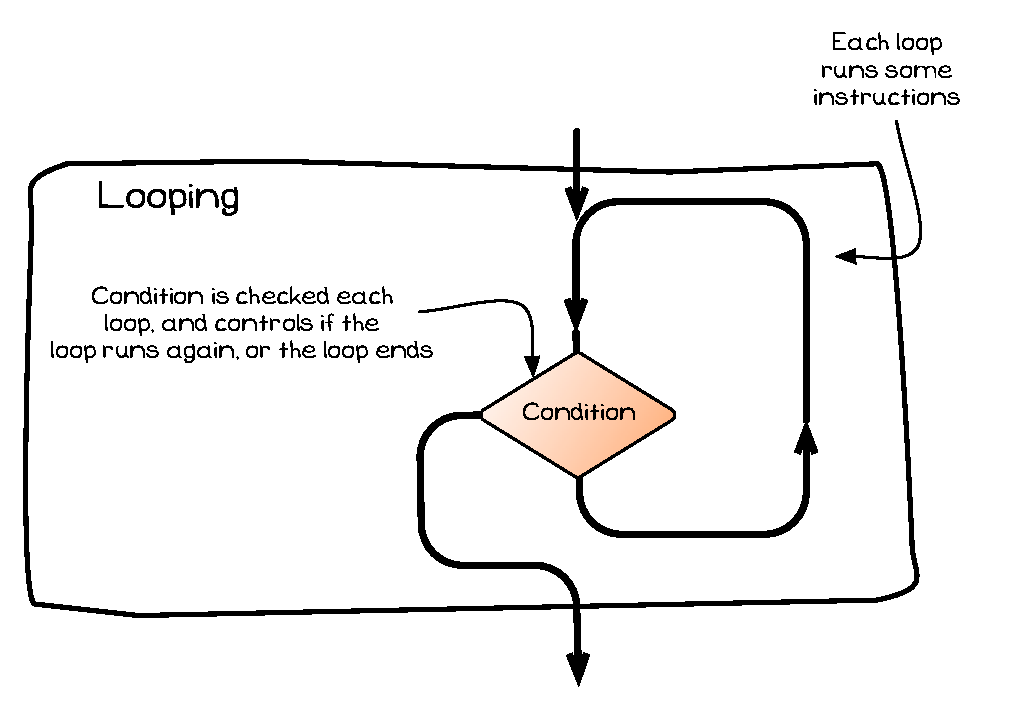
\includegraphics[width=0.9\textwidth]{./topics/control-flow/diagrams/Looping} 
   \caption{Looping commands the computer to repeat a path}
   \label{fig:looping}
\end{figure}

\mynote{
\begin{itemize}
  \item Looping is a kind of \textbf{action}. You can command the computer to repeat the steps within a path.
  \item A number of steps are performed each loop:
  \begin{itemize}
    \item The instructions within the loop are executed.
    \item The \emph{condition} is checked, and the instructions are either run again or the loop ends.
  \end{itemize}
  \item The \emph{condition} may be checked before or after the instructions are executed, giving two kinds of loops:
  \begin{itemize}
    \item \nameref{sub:pre_test_loop}: Repeats instructions 0 or more times.
    \item \nameref{sub:post_test_loop}: Repeats instructions 1 or more times.
  \end{itemize}
  \item As with Branching, the Looping Statements have a single entry and a single exit in keeping with the principles of \textbf{Structured Programming}.
\end{itemize}
}


% subsection looping (end)